% vim:syntax=tex

In this section we describe the design of a case study in which we
compare topic models trained on changesets to those trained on snapshots.
%explore the relationship between ownership and linguistic topics in source code.
We describe the case study using the Goal-Question-Metric approach~\cite{Basili-etal:94}.
The data and source code for the case study is available in this paper's online
appendix\footnote{\textbf{REVIEWER URL ONLY:} \url{http://cscorley.students.cs.ua.edu/cfl/}}.

\subsection{Definition and Context}

% TODO
Our \textit{goal} is to evaluate the usefulness of topic models built
from changesets.
The \textit{quality focus} of the study is on informing development
decisions and policy changes that could lead to software with fewer
defects.
The \textit{perspective} of the study is of a researcher, developer, or
project manager who wishes to gain understanding of the concepts or
features implemented in the source code.
The \textit{context} of the study spans the version histories of fourteen
open source systems.

Toward achievement of our goal, we pose the following research questions:
\begin{description}[font=\itshape\mdseries,leftmargin=10mm,style=sameline]
% TODO
    \item[RQ1] How do changeset-based topic models perform for feature location?
    \item[RQ2] How do \emph{temporal} simulations of changeset-based topic models perform for feature location?
\end{description}
At a high level, we want to determine the feasibility in using changesets
to train topic models for feature location.
In the remainder of this section we introduce the subjects of our study,
describe the setting of our study, and report our data collection and analysis procedures.

%%%%%%%%%%%%%%%%%%%%%%%%%%%%%%%%%%%%%%%%%%%%%%%%%%%%%%%%%%%%%%%%%%%%%%%%

\subsection{Subject software systems}

All of our subject software systems come from two publicly-available
datasets.  The first is a dataset of four software systems by Dit et
al.~\cite{Dit:2013} and contains method-level goldsets.  The second is
a dataset of fourteen software systems by Moreno et
al.~\cite{Moreno:2014} and contains class-level goldsets. The four
software systems in the first dataset also appear in the second,
supplying us with both class- and method-level goldsets for the queries.

% TODO put a table describing systems (how many SLOC, corpus sizes) here
% TODO put paragraph describing each system in english here

%%%%%%%%%%%%%%%%%%%%%%%%%%%%%%%%%%%%%%%%%%%%%%%%%%%%%%%%%%%%%%%%%%%%%%%%

\subsection{Setting}

\begin{figure*}[!th]
    \centering
    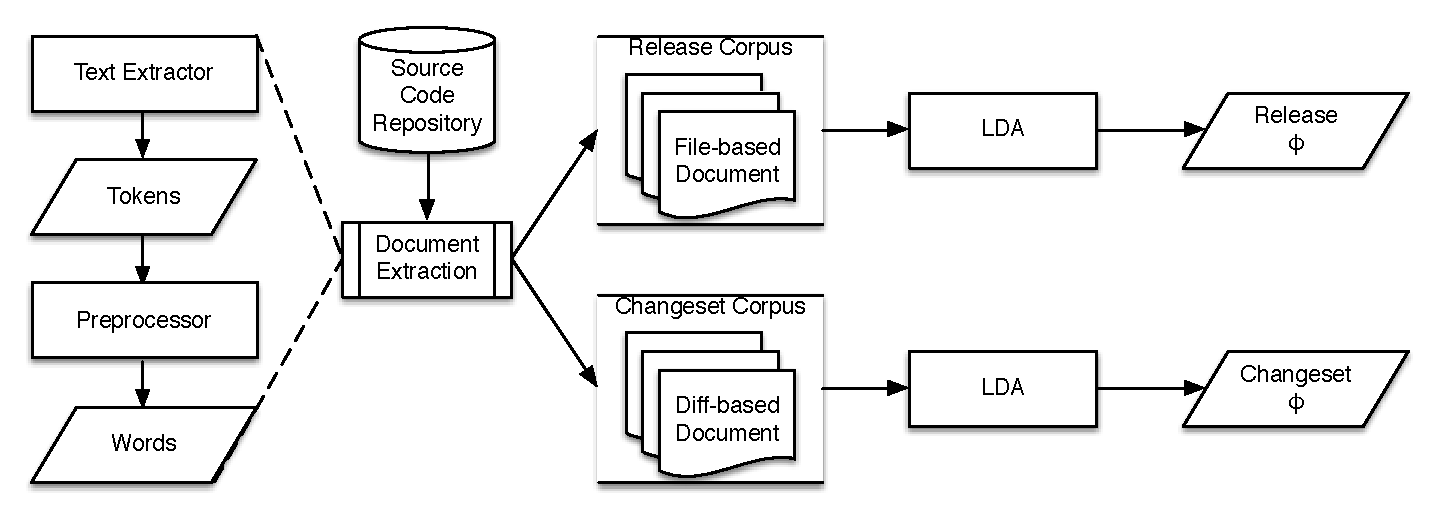
\includegraphics[width=.75\textwidth]{changeset}
    \caption{Extraction and Modeling Process}
    \label{fig:process}
\vspace{-10pt}
\end{figure*}

Our document extraction process is shown on the left side of Figure~\ref{fig:process}.
We implemented our document extractor in Python v2.7
using the Dulwich library\footnote{\url{http://www.samba.org/~jelmer/dulwich/}}. %\footnote{\url{https://pypi.python.org/pypi/dulwich}}
We extract documents from both a snapshot of the repository at a tagged
snapshot and each commit reachable from that tag's commit.
The same preprocessing steps are employed on all documents extracted.

% TODO
For our document extraction from a snapshot, we ...

To extract text from the changesets, we look at the output of viewing
the \texttt{git diff} between two commits.
Figure~\ref{fig:diff} shows an example of what a changeset might look
like in Git.
In our changeset text extractor, we only extract all text related to the
changed file, e.g., context, removed, and added lines.
Metadata lines are ignored.
Note that we do not consider where the text originates from,
only that it is text changed by the commit.\footnote{
The Apache Lucene and Solr projects were merged into a single, new repository
during their development.
We only use changes that affect each project's subfolder in the merged repository,
and also include all changes from the two pre-merge repositories in each project's respective corpus.
}


After extracting tokens, we split the tokens based on camel case,
underscores, and non-letters.
We only keep the split tokens; original tokens are discarded.
We normalize to lower case before filtering non-letters, English stop words~\cite{StopWords}, Java keywords, and words shorter than three characters long.
We do not stem words. \attn{cite reason?}

Our modeling generation is shown on the right side of Figure~\ref{fig:process}.
We implemented our modeling using the Python library Gensim~\cite{Gensim}.
Our evaluation is two-fold: we compare results for both LDA and LSI.

\subsubsection{LDA configuration}

Gensim's LDA implementation is based on an online LDA by Hoffman et al.~\cite{Hoffman-etal:2010}
and uses variational inference instead of a Collapsed Gibbs Sampler.
Unlike Gibbs sampling, in order to ensure that the model converges for each document,
we allow LDA to see each mini-batch $5$ times by setting Gensim's initialization parameter \texttt{passes} to this value
and allowing the inference step $1000$ iterations over a document.
We set the following LDA parameters for all fourteen systems:
$500$ topics ($K$), a symmetric $\alpha=1/K$, and a symmetric $\beta=1/K$.
These are default values for $\alpha$ and $\beta$ in Gensim.

For the temporal evaluation, we found it beneficial to consider two other parameters: $\kappa$ and $\tau_0$.
As noted in Hoffman et al.~\cite{Hoffman-etal:2010}, it is beneficial to
adjust $\kappa$ and $\tau_0$ to higher values for smaller mini-batches.
These two parameters control how much influence a new mini-batch has on the model when training.
However, the implementation of Gensim at the time of this paper did not
include a way to adjust $\tau_0$, so we only adjust $\kappa$.
We chose $\kappa=2.0$ for all systems, because the temporal evaluation
would often have mini-batch sizes in single digits.

\subsubsection{LSI configuration}

% TODO
Gensim's LSI implementation is based on an online LSI by {\v R}eh{\r u}{\v r}ek\cite{Radim:2011}.
We set the number of topics the same as LDA for each project.
The remaining parameters are left at default values, including those used
during the temporal evaluation.

\begin{figure}[ht]
\centering
\footnotesize
\begin{lstlisting}[language=diff, basicstyle=\ttfamily]
diff --git a/lao b/tzu
index 635ef2c..5af88a8 100644
--- a/lao
+++ b/tzu
@@ -1,7 +1,6 @@
-The Way that can be told of is not the eternal Way;
-The name that can be named is not the eternal name.
 The Nameless is the origin of Heaven and Earth;
-The Named is the mother of all things.
+The named is the mother of all things.
+
 Therefore let there always be non-being,
   so we may see their subtlety,
 And let there always be being,
@@ -9,3 +8,6 @@ And let there always be being,
 The two are the same,
 But after they are produced,
   they have different names.
+They both may be called deep and profound.
+Deeper and more profound,
+The door of all subtleties!
\end{lstlisting}
\caption{Example of a \texttt{git diff}. Black or blue lines denote metadata about the change useful for patching, red lines (beginning with a single~\texttt{-}) denote line removals, and green lines (beginning with a single~\texttt{+}) denote line additions.}
\label{fig:diff}
\vspace{-10pt}
\end{figure}


%%%%%%%%%%%%%%%%%%%%%%%%%%%%%%%%%%%%%%%%%%%%%%%%%%%%%%%%%%%%%%%%%%%%%%%%

\subsection{Data Collection and Analysis}

% TODO
We create two corpora for each of our fourteen subject systems.
We then model the documents into topics.

To answer RQ1, we take the traditional approach to evaluation:

\begin{enumerate}
    \item Build a topic model from a corpus
    \item Query the model
    \item Rank the source code entities by how similar their doc-topic is to the query's.
\end{enumerate}

We build a topic model for two corpora:
\begin{enumerate}
    \item Source code entities of a snapshot 
    \item All changesets leading up to the snapshot 
\end{enumerate}

The snapshot-based model is our baseline for comparison in our study.

To answer RQ2, we must take a different approach.
Since both LDA and LSI can be used as online topic models, we can
``simulate'' the results of a feature location technique over time.

Summary:
\begin{enumerate}
    \item Determine which commits to stop at and create mini-batches out of the commits in between
    \item For each mini-batch:
    \begin{enumerate}
        \item Update the model with the new document
        \item Extract a snapshot of the source code at that commit.
        \item Infer from the model the document-topics for each entity in the snapshot
        \item Query the model with the feature request text.
        \item Rank the source code entities by how similar their doc-topic is to the query's.
    \end{enumerate}
\end{enumerate}


However, only the Dit et al. dataset includes traceability links between
the queries and the commits the goldsets are extracted from\footnote{
Authors of \cite{Moreno:2014} did not respond to requests for this data.}.
This limits our temporal study to those four systems.

%%%%%%%%%%%%%%%%%%%%%%%%%%%%%%%%%%%%%%%%%%%%%%%%%%%%%%%%%%%%%%%%%%%%%%%%

\subsection{Results}

% TODO
RQ1 asks ...
